% \input utf8-t1
\documentclass[12pt,a4paper,titlepage]{extarticle}

\usepackage[czech]{babel}
\usepackage[utf8]{inputenc}
\usepackage{fancyhdr}
\usepackage[obeyspaces]{url}
\usepackage[paper=a4paper,top=2cm,left=1cm,right=1cm,bottom=1.5cm]{geometry}
\usepackage{listings}
\usepackage{graphicx}
\usepackage{float}
\graphicspath{ {images/} }
\setcounter{secnumdepth}{0}

\lhead{VUT FIT IVS 2016/2017}
\chead{/dej/uran/dom}
\rhead{Zpráva o~profilování}
\lfoot{}
\cfoot{}

\begin{document}
\pagestyle{fancy}
\section{Zpráva o~provedeném profilování}
Dle zadání bylo nad matematickou knihovnou aplikace provedeno profilování.
Zdrojový kód programu počítající směrodatnou odchylku je uložen v~souboru \path{src/calculator/standard_deviation.py}
vzhledem k~kořenovému adresáři projektu. Tento program je rozdělen do tří funkcí a to:
\begin{description}
\item[main] Funkce pro zkonvertování vstupního toku dat na příslušné datové typy a následné volání směrodatné odchylky.
\item[mean] Funkce, která za použití matematické knihovny spočítá aritmetický průměr hodnot předaných parametrem.
\item[standard\_deviation] Funkce pro samotný výpočet směrodatné odchylky - v~parametru dostane kontejner vstupních hodnot
    a za pomocí \textbf{mean} vypočítá odchylku.
\end{description}

\subsubsection{Python modul cProfile}
Za pomocí utility \path{cProfile} vestavěné ve standardní instalaci jazyka Python jsme provedli měření dle zadání - a to
 10, 100 a 1000 vstupních hodnot. Jedná se o~modul generující jak uživatelsky čitelná data, tak data o~profilování zpracovatelná
 programově - použijeme tabulkovou vizualizaci pomocí IDE \textbf{PyCharm} (ta strojově zpracovatelná budou uložena ve adresáři \path{profiling/profiles/}):
\begin{lstlisting}[language=bash]
$ (for i in {1..10  }; do echo $RANDOM; done) |
    python3 -m cProfile -o sd10.profile     standard_deviation.py
$ (for i in {1..100 }; do echo $RANDOM; done) |
    python3 -m cProfile -o sd100.profile    standard_deviation.py
$ (for i in {1..1000}; do echo $RANDOM; done) |
    python3 -m cProfile -o sd1000.profile   standard_deviation.py
\end{lstlisting}

\subsubsection{UNIX utilita \textit{time}}
Také jsme provedli měření pomocí UNIX utility time s~následujícími výsledky:

\begin{table}[H]
\centering
\begin{tabular}{r|llllll}
\hline
n       & 10    & 100   & 1 000 & 10 000    & 100 000   & 1 000 000  \\\hline
čas[s]  & 00.05 & 00.04 & 00.08 & 00.51     & 04.38     & 33.33      \\
\hline
\end{tabular}
\caption{Měření utilitou \emph{time}}
\end{table}

\subsection{Zhodnocení}
U~interpretovaných jazyků je z~logiky interpretu velké množství zdrojů spotřebováno pro samotnou interpretaci zdrojového programu,
čímž je profilování skriptů tohoto typu velmi ztíženo. Toto tvrzení lze podpořit obrázkem č. 1,
kde se v~prvních 25 modulech/funkcích, které spotřebovaly nejvíce času, \emph{nevyskytuje} žádná matematická operace/funkce -
pouze import matematické knihovny. Většinu času spotřebuje inicializace samotného běhového prostředí pro výpočet,
tedy načtení knihoven, sestavení a naplnění kontejneru vstupních dat atd.

Při vyšším množství vstupních dat (Tabulka č. 1) se začne reálně projevovat asymptotická složitost použitého algoritmu k výpočtu,
odhadem se bude jednat o linerání složitost $O(n)$, což odpovídá i použitým jazykovým konstrukcím (\emph{generator})
v jazyce Python.
\begin{figure}[H]
\centering
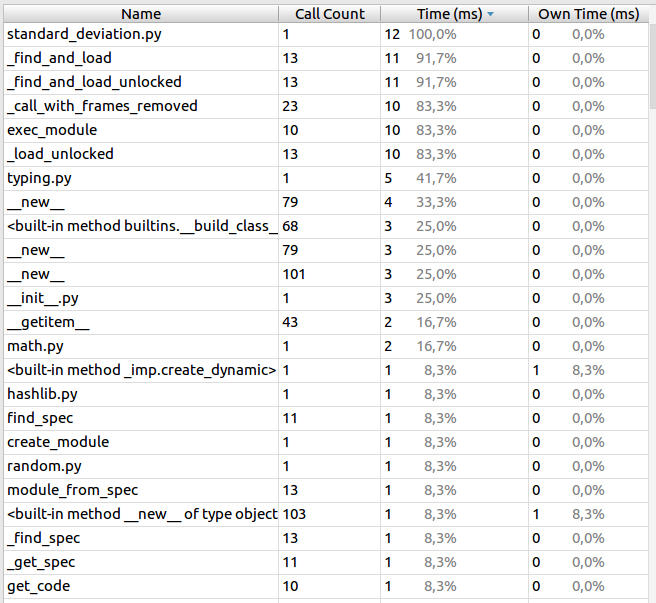
\includegraphics[width=.5\textwidth]{sd10-typehinting}
\caption{Vizualizace zpracování 1000 vstupních hodnot k~výpočtu směrodatné odchylky}
\end{figure}

\subsubsection{\emph{Poznámka}: Dopad použití Python verze 3.6 s~\textit{typehintingem}}
Skript \path{standard_deviation.py} vznikl nejprve v~podobě, kdy používal \textit{typehinting} u~parametrů metod,
kde se v~extrémních případech projevovala režie těchto typů až k~polovině času běhu skriptu. Považujeme to za daň u~tohoto
způsobu implementace \textit{typehintingu} v~jazyce Python, kdy jsou tyto meta-informace zpracovávané samotným interpretem,
jakožto normální zdrojový kód algoritmů a dalších jazykových konstrukcí.

\textit{Typehinting} byl tedy ze skriptu odebrán, přestože i nadále jej používá matematická knihovna (pro automatické
napovídání kalkulačky či jednodušše snažší vývoj). Porovnání lze vidět na obrázku č. 2.

\begin{figure}[H]
\centering
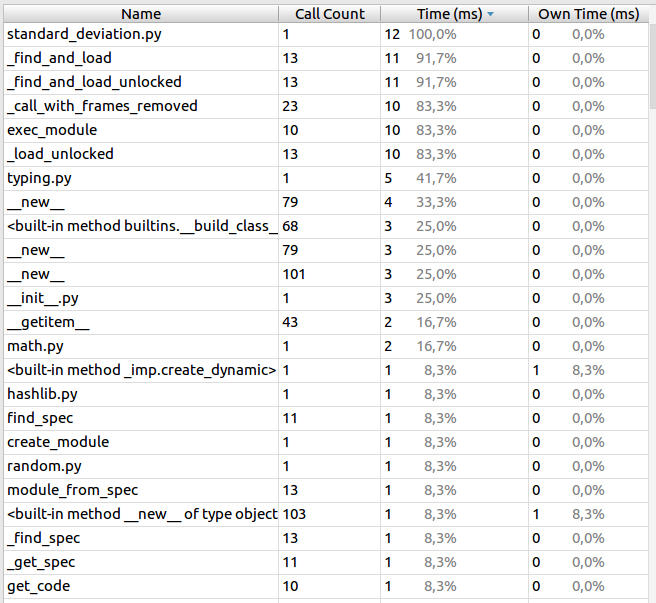
\includegraphics[width=.5\textwidth]{sd10-typehinting}
\caption{Výstup z~odchylky z~desíti hodnot s~aplikovaným \textit{typehintingem} pro porovnání}
\end{figure}

\end{document}
